\capitulo{4}{Técnicas y herramientas}

Apartado cuyo objetivo es presentar las técnicas metodológicas y las herramientas de desarrollo que se han utilizado para llevar a cabo el proyecto. Si se han estudiado diferentes alternativas de metodologías, herramientas, bibliotecas, etcétera.\\

Se comenta los aspectos más destacados de cada opción, con un repaso somero a los fundamentos esenciales y referencias bibliográficas para que el lector pueda ampliar su conocimiento sobre el tema.
\section{¿Por qué Python?}
La razón es la sencillez y capacidad de este lenguaje para el análisis y tratamiento de los datos, gracias a librerías como Pandas o Numpy. Base gran parte de la metodología de análisis usada en este proyecto en el libro: Python for Data Analysis. \cite{analisis}
\\ 
Las distintas posibilidades cotejadas antes de empezar fueron: Java, Android, R y Python. El primero en ser descartado fue Java, tras un estudio inicial sobre como se quería desarrollar la aplicación. Después de buscar entre diferentes fuentes; Java no era la mejor opción, dichas fuentes siempre te orientaban hacia Python y/o R, debido a la cantidad de librerías enfocadas al análisis y tratamiento de los datos que estos poseen.\\
La razón por la que se planteo Android fue por que este trabajo está desarrollado para unir el mundo de la dietoterapia, y las ciencias de la Salud con la informática. La forma más clara y rápida de llevar al usuario dichas tecnologías es a través de un  SmartPhone, pero se acabó descartando debido a la falta de conocimientos sobre sistemas Android. A estas alturas ya solo existían dos opciones:  Python y R.\\
Tras indagar superficialmente sobre ambos lenguajes para el análisis y el tratamiento de datos, se llego a la conclusión que ambos lenguajes tienen una forma de trabajar muy similares,y  debido a que durante los años de estudio el alumno ha trabajado en numerosas ocasiones con Python, se decantó por Python.
\section{Metodología}
\subsection{Introduccón}
En este apartado se explicará el cómo y porque se ha tratado los datos en este trabajo,  además de los diferentes cálculos internos que se realizan para el sistema de recomendaciones, cálculos, etc.
\subsection{Excell y Pandas}
Se ha usado la herramienta de Microsoft Excel, para simular una base de datos, trabajando los datos en formato DataFrame. Los DataFrame son proporcionados por la librería Pandas. Existen diferentes hojas de cálculo, que funcionan como colecciones de una base de datos. Estas hojas son explicadas más adelante.
\subsection{DataFrame}
Se usan los DataFrame, para llevar un registro de todos los datos que el programa necesita, se tiene en cuenta tanto las bases de datos de los alimentos, usuarios y comidas como lo que el usuario lleva en el día.
\\
Los alimentos se tratan en el momento en el que se registra el usuario, de manera que se separan las comidas de la lista principal, creando 5 listas (Desayuno, Merienda, Comida, Almuerzo y Cena), se tratan por separado y se filtran. Cada modificación o inserción de un dato o usuario se hace sobre el DataFrame, el cual sustituirá a la base de datos durante el guardado.

\section{Técnicas}
\subsubsection{Introducción}
En este apartado se hablará de manera breve de las técnicas usadas durante el proyecto, y la razón por la que se escogieron dichas técnicas. Posiblemente haya argumentos repetidos en otros apartados similares, por lo que se expresará exclusivamente finalidad y razonamiento.
\subsection{Aprender a aprender}
\begin{quote}
“Aprender a aprender supone disponer de habilidades para iniciarse en el aprendizaje y ser capaz de continuar aprendiendo de manera cada vez más eficaz y autónoma de acuerdo a los propios objetivos y necesidades.\\

Esta competencia tiene dos dimensiones fundamentales. Por un lado, la adquisición de la conciencia de las propias capacidades (intelectuales, emocionales, físicas), del proceso y las estrategias necesarias para desarrollarlas, así como de lo que se puede hacer por uno mismo y de lo que se puede hacer con ayuda de otras personas o recursos. Por otro lado, disponer de un sentimiento de competencia personal que redunda en la motivación, la confianza en uno mismo y el gusto por aprender. Significa ser consciente de lo que se sabe y de lo que es necesario aprender”. \cite{aprenderAAprender}


\end{quote}

Es decir, el autoaprendizaje no solo ayuda al usuario a aprender de manera autónoma, sino que le ayuda a que todo aquello que ha conseguido, para el sea, de alguna forma, una meta, algo que lograr, algo suyo, que no se le va a olvidar tan fácilmente, como información memorizada, sino que será el resultado de pequeños logros personales que integrarán al usuario, una nueva información, como si fuese suya.
\subsection{Tasa Metabólica Basal - TMB}
La tasa metabólica basal (TMB) es el gasto calórico de una persona a lo largo del día. A este cálculo se le multiplica un valor relacionado con la actividad física del usuario  y como resultado tenemos las kilocalorías diarias que el usuario gasta al día o lo que es equivalente, que el usuario debe tomar para mantenerse en su peso.\\
El cálculo es genérico, por esta razón es un método cada vez más en desuso. Aun así, sigue siendo un de los métodos más utilizados para la recomendación dietética por especialistas en la materia.\\
La fórmula del TMB es la siguiente:\\
\textbf{Hombres:}
\begin{equation}
TMB =  ((10 * Peso(kg))+(6,25*Altura (cm))-(5*edad)+5)*ActividadFisica
\end{equation}
\textbf{Mujeres:}
\begin{equation}
TMB =  ((10 * Peso(kg))+(6,25*Altura (cm))-(5*edad)-161)*ActividadFisica
\end{equation}
Donde actividad física se corresponde con los siguientes valores mostrados en la Tabla \ref{tabla:TablaActividadYMB}. \cite{TMB}
\tablaSmall{Valor de la actividad física en TMB}{l c c c c}{TablaActividadYMB}
{ \multicolumn{1}{l}{Ejercicio } & Valor de ActividadFisica\\}{ 
Poco ejercicio & 1,2\\
Ejercicio ligero(1-3 dias/semana) & 1,35\\
Ejercicio Moderado (3-5 diás/semana) & 1,55\\
Ejercicio fuerte (6-7 dias/semana & 1,725\\
Ejercicio muy fuerte (dos veces al día) & 1,9 \\
} 
Para cumplir el objetivo de la persona (subir o bajar de peso), se suele añadir o restar un valor estandarizado. Este valor se encuentra entre 300 y 500 calorías si se quiere adelgazar o subir aproximadamente un kilogramo por semana \cite{TMBadiccional}. \\
Es este proyecto para evitar la generalización de la fórmula, lo cual es la principal razón de que la fórmula este siendo sustituida por la toma de medidas corporales, se crea una variable que inicialmente empieza en 500 calorías, pero que varía en base al progreso del peso del usuario. Si el usuario se pasa o se queda corto del objetivo normal (con un rango de error del 15\%), este valor variará ajustándose cada vez más al usuario (si el usuario se excede se le reducirán 50 calorías, si se queda corto se le sumarán 40).\\

\subsection{Tratamiento de Excepciones}
A través del tratamiento de excepciones, y con el uso de la librería \textbf{messagebox} se informa al usuario de las distintas situaciones que se pueden dar durante el uso del programa. Existe tres tipos principales de cuadros de textos, que emergen informando al usuario de algún tipo de problema o simplemente de que una acción ha finalizado correctamente.\\


\textbf{Información}\\

\begin{figure}[h]
\centering
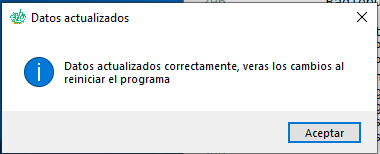
\includegraphics[scale=1]{Informacion} 
\caption{Ventana emergente de información}
\end{figure}
Muestra la información de que un proceso ha concluido correctamente. También explican si el usuario ha de realizar algo una vez terminado el proceso para que termine la completa finalización de este.\\


\textbf{Aviso}\\

\begin{figure}[ht]
\centering
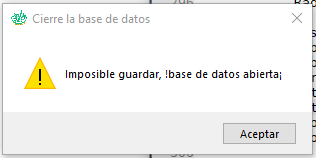
\includegraphics[scale=1]{Aviso} 
\caption{Ventana emergente que avisa que una acción no se ha podido realizar.}
\end{figure}
Pantalla que advierte que algo no ha salido bien. El usuario puede seguir con el uso del programa, pero si quiere realizar la acción que estaba realizando, deberá seguir las instrucciones proporcionadas en el cuadro de aviso.\\
\clearpage
\textbf{Error}\\

\begin{figure}[ht]
\centering
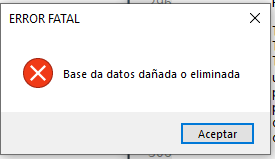
\includegraphics[scale=1]{Error} 
\caption{Ventana emergente que muestra que ha ocurrido un Error.}
\end{figure}
Pantalla que advierte de un error grave, en el que se ha corrompido la estructura de datos del programa.\\

A través de estos cuadros se traduce los diferentes problemas que puedan surgir en la utilización del programa; de manera gráfica y entendible por el usuario, haciendo el funcionamiento de este lo más transparente al usuario posible.
\subsection{Diseño}
Diseño simple, se evita crear extensos árboles de ventanas y frames, creando una navegabilidad sencilla e intuitiva. Debido al principal objetivo del proyecto,  esta aplicación está orientada a todos los públicos, por lo que se procura que la interfaz sea simplista, y fácil de entender.\\

Se basa en un menú principal ramificado en tres vertientes: Usuario, Dieta y Registro (en el programa aparecen con otros nombres). En la vertiente usuario, esta la información del usuario y la posibilidad de cambiar dichos datos para un avance del programa. En la rama de la dieta se encuentra el tronco principal de la aplicación, se muestra las recomendaciones alimenticias, a parte de darte libertad a la hora de escoger y decidir que deseas comer en el día de hoy. Por último estaría el registro o historial, es decir, todo aquello que necesites para llevar un registro de tu progreso y concienciar de esta manera al usuario.\\

Respecto a los colores, se decido un tema básico que no agote la vista del usuario, ni tenga múltiples colores deslumbrantes, da la posibilidad al usuario de elegir entre una serie de estilos predefinidos para que escoja el que mejor se ajuste a sus gustos y necesidades.\\
\section{Estructura del programa}
\subsection{Introducción}

La estructura es una variación del modelo-vista-controlador, separando el módulo HealthApp (que funciona de Main), del resto de módulos, que son los que implementan la estructura CAV (Cálculos, Administración y Vista).
\begin{enumerate}
\item	\textbf{HealthApp} – Tronco del programa
\item	\textbf{Vistas} – Relacionado con la parte visual
\item	\textbf{CalculosDieta} – Todo cálculo usado en el programa
\item	\textbf{AdminBase} – Todo proceso relacionado con la base de datos

\end{enumerate}

\subsection{Cálculos, Administración y vista}
Podríamos llamar propiamente a este modelo el CAV, y se basa en separar toda función que se vaya a crear en el programa en estos tres pilares. \\
Cada vez que la lógica de una función necesitaba un hueco donde encajar y ninguno de los módulos creados lo sostenía, se iba creando un nuevo módulo. Debido a la forma de trabajar del alumno, la estructura acabó cogiendo esta forma.  Por un lado, todo elemento relacionado con la base de datos, por otro lado todo cálculo matemático realizado en el programa y por último toda función que intervenga en la interacción usuario-aplicación.\\

Para crear una estructura, y no tener un código modular sin coherencia, se llevó a cabo una serie de reglas sencillas:
\begin{itemize}
\item	Si su finalidad es puramente visual – Vista
\item	Si realiza cálculos u operaciones matemáticas, indistintamente de si sea sobre la dieta -CalculosDieta
\item	Si interacciona y guarda datos en la base de datos -AdminBase
\item	Si mezcla alguna de estas funcionalidades, por ejemplo, guardar en la base de datos y mostrar por pantalla algo, se tendrá en cuenta cual es su principal finalidad, por ejemplo, se guardan estilos que se cargaran automáticamente para el diseño del programa, obviamente su finalidad es puramente visual, y guardar en la base de datos una transacción necesaria.
\item	Cualquier objeto, ventana, tabulación, etc. Que siempre vaya estar ahí al HealthApp, pero sus modificaciones se repartirán entre los diferentes módulos.

\end{itemize}
Estas reglas, a día de hoy, han cumplido con todas las funciones que se han creado en el programa dando el resultado previsto.
\section{Librerías}
\subsection{Pandas}
La librería desarrollada por Wes McKinney, Pandas, es una librería usada para el tratamiento de los datos como estructuras. Debido a que este proyecto se enfoca en el análisis de datos, y no en el tratamiento de bases de datos, se decidió crear una base de datos local en un archivo Excel.\\
La primera opción fue la librería “openpyxl”, la cual es una librería de código abierto, que permite la carga y manejo de datos ".XLS". De esta manera se  cargaba los datos, pero en listas desestructuradas que complicaban el posterior análisis de la información.\\
Acto seguido basándose en el libro: Python for Data Analysis \cite{analisis}, se decidió probar con Pandas, esta librería permitía leer los datos de los archivos ".xlsx", en forma de DataFrames. Simplificando el análisis de los datos, permitiendo tratarles tanto como DataFrames como en forma de vectores.
\subsection{Numpy}
Como se ha nombrado anteriormente, el libro: Python for Data Analysis \cite{analisis}; Hace especial énfasis en la conveniencia del uso de Numpy para el tratamiento y análisis de los datos. Es la principal librería sobre la que se ha  trabajado a lo largo de la carrera en cuanto a análisis de datos en Python, y una de las mas recomendadas por varias fuentes de información. La librería Numpy es la encargada, del tratamiento, procesamiento y cálculo de todos los datos que internamente realiza el programa.
\subsection{Interfaz Gráfica}
La librería utilizada para realizar y diseñar la interfaz gráfica fue Tkinter, tras indagar en diferentes fuentes, se decantó por Tkinter debido al desconocimiento sobre el funcionamiento de interfaces gráficas con Python. Entre las opciones que se barajaron se encontraban: Tkinter, WxPython, PyQt y PyGTK.\\

Tkinter presentaba una serie de ventajas: viene preinstalada con Python, es fácil de aprender y además cuenta con una documentación amplia y extensa. Pero entre sus desventajas, se encuentran: la escasez de recursos gráficos, la sencillez implica poca variedad de elementos y funciones (complicando en numerosas ocasiones la navegabilidad) y la lentitud que este tiene debido a que dibuja cada elemento sobre cada pantalla, en tiempo de ejecución.\\

La segunda opción que se planteo, fue WxPython. Presentaba  grandes ventajas como: la rapidez,  la flexibilidad que este ofrecía y la variedad opciones que tiene para crear una interfaz gráfica compleja. Después de ser meditado se llego a la conclusión de que todo lo que  ofrecía WxPython, era innecesario para la interfaz tan simplista que necesitaba el proyecto, y el aprendizaje era más complejo, además de tener recursos limitados, y tener menor cantidad de documentación al alcance del alumno. Su mayor inconveniente es que tiene una comunidad muy activa, la cual está constantemente insertando cambios y creando problemas de compatibilidad.\\

El resto de librerías fueron descartadas, al poco de buscar información sobre ellas puesto que daban las mismas ventajas o similares que la WxPython, pero tenían mas inconvenientes, al menos para el tema que aborda este proyecto.
\subsection{MatplotLib}
Librería de Python extendida en su uso, para el análisis y representación de los datos. Se utiliza a lo largo del proyecto para crear diferentes gráficos e histogramas para dar una perspectiva más visual de los resultados al usuario.
\subsection{Pillow}
Usada en su versión 6.0. Es una librería que permite la carga y posterior muestra de imágenes en una aplicación Python. Es usada en numerosas ocasiones a lo largo del proyecto, para visualizar el logotipo, o diferentes imágenes guía que ayudan al mejor entendimiento del programa.
\subsection{webbrowser}
Módulo que proviene de una interfaz de alto nivel para mostrar archivos web a los usuarios.
\subsection{os}
Librería utilizada durante el proyecto para la carga del manual en PDF por parte del programa. Es una librería cómoda que permite acceder y mostrar varios elementos que se encuentran en el sistema.
\subsection{datetime}
Librería normalmente preinstalada con Python, que da un control sobre la fecha y la hora del sistema. Sumamente útil para el control de registros  e historial.

\subsection{auto-py-to-exe}
No es usada durante el desarrollo del proyecto, pero si al finalizar dicho desarrollo para crear un archivo ejecutable (.exe). Utiliza internamente la librería pyinstaler, y hace uso de la librería Tkinter para otorgar una interfaz gráfica al comando pyinstaller, haciendo más fácil su uso.

\section{Módulos}
\subsection{Cálculos Dieta}
Módulo encargado de los cálculos del programa. En el se encuentra el motor del sistema de recomendación, encargándose de:
\begin{itemize}
\item Calcular la calidad de los alimentos en base a sus características.(Algoritmo Nutriscore)
\item Calculo y reajuste de la Tasa Metabólica Basal (TMB)
\item Reparto de kilocalorías y los diferentes macronutrientes, teniendo en cuenta la comida del día y las necesidades que este aplica.
\item Aplicación de la formula del sistema de recomendación
\end{itemize}

\subsubsection{Reparto Calórico entre comidas.}
Como se aprecia en la Tabla \ref{tabla:porcentaje}, se tiene en cuenta no solo la carga calórica en cada comida, sino la distribución de este porcentaje entre los distintos nutrientes. (Consultar Tabla \ref{tabla:distribucionDietas})\\

\tablaSmall{Porcentajes totales de cada comida}{l c c c c}{porcentaje}
{ \multicolumn{1}{l}{Comida } & Porcentaje(\%) & Descripción\\}{ 
Desayuno & 24,75 & Alta carga calórica, rica en hidratos\\
Almuerzo & 13,5 & Baja carga calórica.\\
Comida & 30,5 & Mayor carga calórica, eje central.\\
Merienda & 11,5 & comida de paso y casi prescindible.\\
Cena & 19,75 & Alta carga calórica pero con moderación.\\
} 
Se calcula el número de Kilocalorías que se tiene que tomar de hidratos, grasas y proteínas, en base al tipo de dieta recomendable para su patología.\textbf{distribuciónDeMacronutrientes} toma como parámetros las kilocalorías diarias calculadas previamente por la función calculoTMB, y el tipo de dieta del usuario en base a su patología, y te devuelve una lista de los macronutrientes diarios, repartidos en gramos y las kilocalorías totales en el siguiente orden: ListMacDiarios [Kilocalorías, Hidratos, Proteínas, Grasas].

\subsubsection{Formula del Sistema de recomendación}
Motor del sistema de recomendación. A través de la formula:
\begin{equation}
DiferenciaMacronutriente = \frac{(KMCD - A)}{((KCDT-KMM)+(KMTC-KTM))}
\end{equation}
Donde:
\begin{itemize}
\item \textbf{KMCD:} Número de Kicalorías del macronutriente (Hidratos, proteínas o grasas) de la Comida (Desayuno, almuerzo...) que debería llevar en esa comida
\item \textbf{A:} Actual número de kicalorías de ese macronuetriente que llevo en todo el día (Si estoy en Comida: desayuno+almuerzo+comida).
\item \textbf{KCDT:} Kilocalorías que debería comer en esta comida concreta para este macronutriente concreto.
\item \textbf{KMM:} Kilocalorías del macronutriente concreto del menú.
\item \textbf{KMTC:} Kilocalorías totales que debería comer en esta comida.
\item \textbf{KTM:} Kilocalorías totales que tiene el menú a recomendar.

\end{itemize}
La fórmula es el eje central del filtro de recomendación basado en contenidos. Se evalúan diferentes características de los tres aspectos claves a la hora de la recomendación según este proyecto: Usuario, Alimento, y el momento del día.\\
De esta manera cuanto mayor sea la diferencia entre lo que debo llevar y lo que llevo comido, y menor sea la diferencia entre lo que deseo y las características del alimento, mayor será la puntuación de ese alimento para su recomendación ( \textbf{Nota: Se ordena de mayor diferencia a menor}).\\
Por último, se realiza la media entre los tres macronutrientes principales:
\begin{equation}
DiferenciaTotal = \frac{(Diff.Hidratos+Diff.Proteina+Diff.Grasas)}{3}
\end{equation} 
En el caso de que algún macronutriente dé negativo, no se tendrá en cuenta.


\subsection{AdminBase y estructura de la base de datos}
En este apartado se expone la estructura la base de datos y de como se cargan, guardan y trabajan los datos desde el módulo \textbf{AdminBase}, el cual, es el encargado del manejo de los datos, y la traducción con el sistema de archivos.
\subsubsection{CargaBaseDeDatos y guardaDatos}
Estas dos funciones cargan y guardan los datos de/en la base de datos respectivamente. Nada más iniciar la ejecución del programa, almacena los datos leídos de la base de datos, en una serie de DataFrames independientes. Se trabaja con cada uno de ellos sin tener en cuenta al resto y se guarda el resultado de los cambios producidos durante la ejecución del programa, sustituyendo la base de datos por los DataFrames. \\

\subsubsection{Estructura de la base de datos}
La base de datos es almacenada en diversas hojas de cálculo, simulando de esta manera diferentes colecciones de una base de datos. Estas colecciones serias:\\
\textbf{\textsc{ALIMENTOS}}\\
La hoja de alimentos, es una hoja de menús ya construidos. Esta hoja consta de doce campos:\\
La clave primaria de esta colección es el nombre del menú. Los campos son:
\imagen{A}{Estructura base de datos alimentos}
Nombre (Único), Calorías, Grasa, Saturadas, Hidratos, Fibra, Azúcares, Proteínas, Sodio, Tipo, LRE(Last Reciently Eat) y Calidad.
Los primeros diez campos son las diferentes características del menú, mientras que los otros tres son parte de la gestión de dichos menús.\\
El tipo marca el tipo de comida que es, un mismo menú puede ser a la vez desayuno, almuerzo y merienda, cena y comida, etcétera. Por ello se planteo dos posibilidades.
\begin{enumerate}
\item Cadena de carácteres, con la combinación de la inicial o nombre de las diferentes combinaciones de tipos de comida y la posterior separación de estas. Esto dio diversos problemas con la carga y filtrado de los datos.
\item Cadena de bits: desayuno-almuerzo-comida-merienda-cena, donde el valor 1 sería si es valido para esa comida y 0 si no lo es.
\end{enumerate} 
Se decidió escoger la segunda opción. Una vez creado los métodos que traducen el sistema numérico en una cadena de bits, el tratamiento en conjunto de las combinaciones como un simple número simplificó las cosas. Ejemplo:
1-1-0-1-0 \\
Significa que es desayuno, almuerzo y merienda, pero no comida o cena, luego esto se traduce en el número decimal, que en este caso sería 26.\\

El LRE lleva una métrica de la frecuencia con la que el usuario toma esa opción, literalmente significa “last reciently eat” (El más reciente ingerido), que en este caso hará de contador. En la expansión del proyecto (Explicado en el apartado 7), este dato sería el único encontrado de manera Local, ayudando a personalizar aún más la aplicación para una mejor experiencia de usuario. \\

La Calidad, como el propio nombre indica, es la calidad del alimento, es la variable que marca la diferencia entre 100 kilocalorías de ensalada y 100 kilocalorías de azúcar. Tiene un rango de valores de la A a la E, siendo A una comida saludable, y E una comida poco recomendable. Internamente el programa lo trata de forma numérica. Este valor se halla a través del algoritmo Nutriscore.

\textbf{\textsc{Usuarios}}\\
La hoja de usuarios alberga los datos de todos los usuarios que usan la aplicación. Está estructurada de forma que contenga los datos principales del usuario, así como, los datos necesarios para el sistema de recomendación. \\
\imagen{BaseUsuarios}{Estructura base de datos Usuarios}
La clave primaria sería el DNI del usuario, el cual, se encuentra dentro del campo ID. La hoja se estructura de la siguiente manera:\\
Id (PK)-nombre-apellido-password-sexo-edad-altura-peso-actividad-patología (FK de la tabla Patologías) y tipo.\\
Tanto \textbf{id, como nombre, apellido y password}, son los datos privados del usuario, los cuales, son simplemente informativos y no tienen ningún valor adicional en el cálculo de la dieta y los resultados. En cambio, \textbf{el sexo, la edad, altura, peso, actividad, patología y tipo, influyen de manera directa con el cálculo de la dieta} . A tener en cuenta, que el valor del campo patología es numérico para mayor privacidad y conexión con la base de datos de Patologías, pues es el id de cada patología. En el caso de valer -1, significa que el usuario no tiene ningún tipo de patología y su uso es exclusivamente para el aprendizaje y seguimiento de la dietoterapia adecuada. La actividad tiene valores entre 0 y 4, donde cero significa el máximo nivel de sedentarismo y 4 el máximo nivel de actividad. Por último el tipo, hace referencia, a los objetivos que el usuario tiene respecto a si mismo, si quiere mantenerse, subir de peso, o bajar.\\

\textbf{\textsc{Patologías}}\\
En esta hoja, la cual se encuentra dentro de las BaseDeDatosDeAlimentos, está la información básica de las patologías: \textbf{nombre}, \textbf{id}, y el \textbf{tipo} de dieta que lleva alto o bajo en carbohidratos, proteínas o grasas. Esto se carga al inicio del programa, se comprueba si el usuario padece alguna patología y se selecciona el tipo de dieta correspondiente.\\
\begin{figure}[htb]
\centering
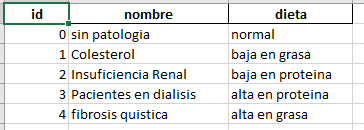
\includegraphics[scale=1]{Patologia} 
\caption{Estructura base de datos Patologías}
\end{figure}

\textbf{\textsc{Registro}}\\
Base de datos que se encuentra en la ruta: assets/RegistroMejora.xlsx, y se encarga de llevar un registro de la mejora del usuario en la aplicación. Esta base de datos guarda los datos imprescindibles para el ajuste de la formula del TMB respecto al usuario concreto.\\
En el momento que un usuario se registra, tiene tres posibilidades de tipo de dieta:
\begin{enumerate}
\item \textbf{bajar:} Se crea un valor inicial igual a -500
\item \textbf{Mantener:} Se crea un valor inicial igual a 0
\item \textbf{Subir:} Se crea un valor inicial igual a 500. 
\end{enumerate}
El valor inicial a la hora del registro es el suplemento que se añade al resultado de la formula del metabolismo basal, para que las calorías a ingerir por el usuario sean las necesarias para lograr el objetivo que se ha propuesto a través del tipo de dieta.
Esta base de datos se estructura de la siguiente manera:
\begin{figure}[htb]
\centering
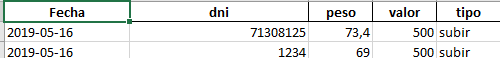
\includegraphics[scale=1]{registroMejora} 
\caption{Estructura base de datos Registro}
\end{figure}
Esto se debe a:
\begin{enumerate}
\item \textbf{Fecha:} Guarda la última vez que se editó la información. De esta manera se puede calcular el peso que se debería haber progresado hasta dicha fecha. No admite cambios de menos de una semana, pues el resultado podría alterar el ajuste del valor.
\item \textbf{dni:} DNI del usuario para saber de quién es el registro que se está llevando.
\item \textbf{Peso:} El peso de la última vez que el usuario edito la información respectiva a su peso. Esto ayuda al seguimiento de la dieta y sus objetivos.
\item \textbf{Valor:} Valor que más tarde se suma al cálculo TMB y que ayuda a cumplimentar mejor su objetivo.
\item \textbf{tipo:} Tipo de dieta u objetivo de la dieta del usuario. Sirve para saber si el usuario a cambiado de objetivo y en caso de no hacerlo, ver cómo va el progreso del usuario.
\end{enumerate}

\subsection{Vista}
En el módulo vista se almacena toda función que tendrá influencia en lo que el usuario ve, es decir:
\begin{enumerate}
\item Actualización de pantallas,
\item Muestra de datos,
\item Transacciones entre ventanas,
\item Actualización de los gráficos,
\item Etcétera.
\end{enumerate} 


\subsubsection{Reconstrucción de frames}

Cada vez que se selecciona una opción, el resto de las opciones cambian aplicándose el sistema de recomendación programado. Se van ajustando las opciones a las necesidades del usuario. Tkinter no dispone de ningún método eficaz que permitiese actualizar un Frame. Por ello, cada vez que se selecciona una opción, se crea un nuevo frame que sustituye al actual, llamándose de manera recursiva con distintas opciones sobre el sistema de recomendación.\\

Para evitar errores de coherencia el programa solo actualizará aquellos Frames no bloqueados por el método seleccionar, sacrificando un pequeño porcentaje de la precisión, para conseguir un funcionamiento más fluido sin errores de compatibilidad o múltiples selecciones.\\
\subsection{HealthApp}
Es la columna vertebral del programa, el cual, se encarga de cargar y procesar toda la información relevante que más adelante se va a ir editando en el programa. HealthApp tiene una única función y el resto se divide en clases que se instancian en esta función.\\

Hace de flujo de entrada y salida, donde una condición simula un interruptor permitiendo que la aplicación original, distribuida en clases, se lance o se cierre.\\

Todo se basa en una  jerarquía de objetos, en el que el objeto principal (Menú principal), contiene otros tres objetos que estos a su vez contienen otros, creando una simple estructura de árbol, entendible por cualquier programador. \\

Se crea una clase por tipo de comida barajada. Por lo que cada vez que se crea de manera recursiva el mismo Frame, se está instanciando la clase contenida.

\section{Herramientas}
 Nos centraremos en mencionar de manera breve, las herramientas que se han usado para el desarrollo del programa.
\subsubsection{Anaconda}
Distribución de código abierto, la cual, está indicada para el análisis, procesamiento y computo de datos, de Python y R, trae consigo una serie de programas y características entre los que destacaremos: Spyder y VisualCode.\\

Se decidió usar anaconda, debido a su principal función, el análisis, procesamiento y computo de los datos.
\subsubsection{Spyder}
Spyder es un entorno de desarrollo incluido en el paquete de anaconda.\\

Antes de empezar se probaron varios entornos como: NoteBook, PyCharm, VisualCode y eclipse (añadiendo el API de Python), pero se acabó decantando por Spyder.\\

\subsubsection{GitHub}
Proyección de la metodología GIT para el almacenamiento y control de versiones, sin duda GIT es actualmente la estructura más usada en el mundo de la programación, y GitHub, una de las herramientas más conocidas y valoradas que hay.
\subsubsection{GitKraken}
Potente interfaz gráfica multiplataforma desarrollada por Electron, que nos permite controlar de forma sencilla y cómoda nuestro repositorio GitHub, permitiendo que el uso y control del GitHub fuera más ameno y rápido, sin duda es una de las mejores aplicaciones que he probado, y de las que más me han ayudado a lo largo del proyecto.
\subsubsection{MakeText}
Herramienta de escritorio, utilizada para la preparación de documentos en LaTex. Fue utilizada durante el desarrollo del proyecto para plasmar las memorias y anexos, que formarían la documentación del proyecto.